\section{Virtual CED}
\label{sec:chapter_4_section_2}
Il progetto di modellazione di un Virtual CED (Centro Elaborazione Dati) sviluppato presso SOGEI, \`e stato realizzato con
l'intento di avere un modello 3D navigabile per consentire di sviluppare un sistema di Indoor Mapping e Indoor Navigation.
Sono stati sviluppati dei \emph{Plugin} coerenti con il contesto, che hanno portato alla realizzazione in un
Virtual CED mostrato nella Figura~\ref{fig:virtualCED} nella sua vista 3D.\\

\begin{figure}[htbp] %  figure placement: here, top, bottom, or page
   \centering
   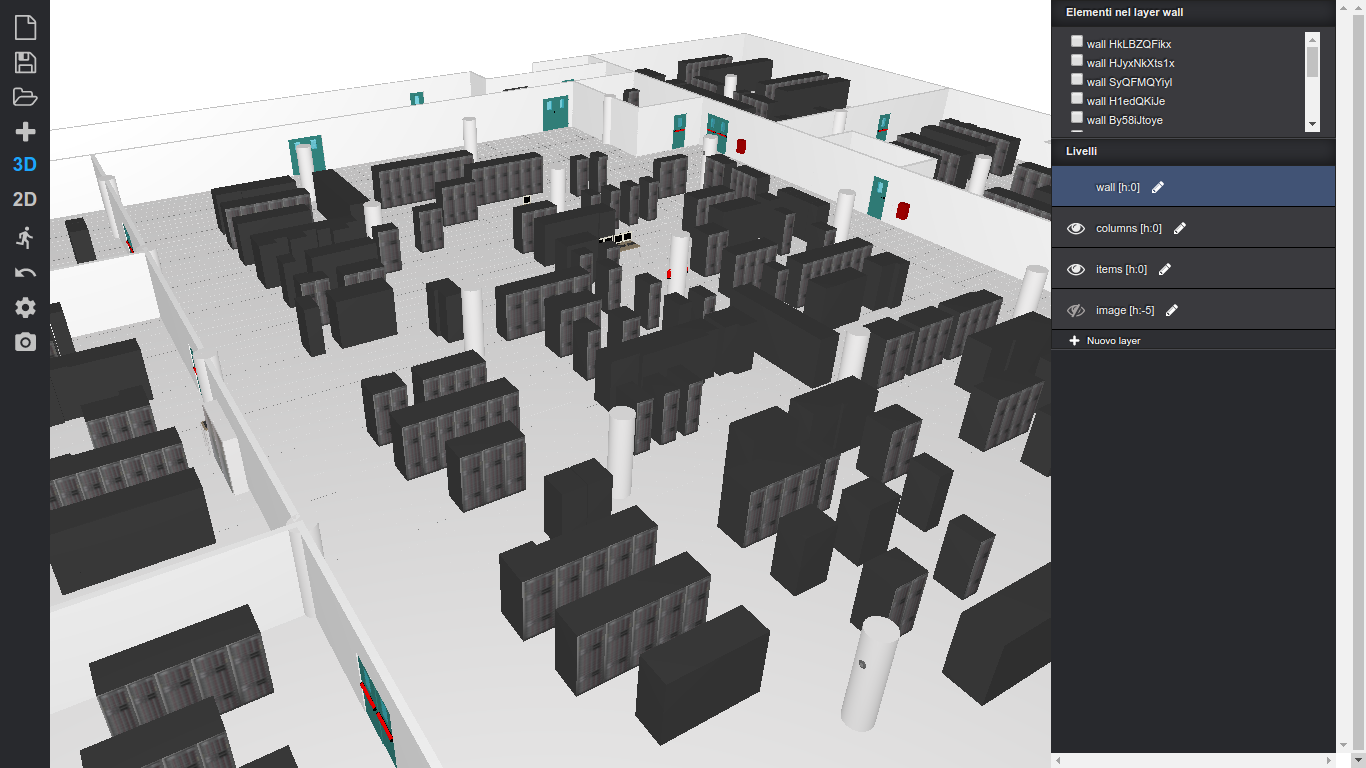
\includegraphics[width=1\linewidth]{images/virtualCED}
   \caption{Vista 3D di un Virtual CED}
   \label{fig:virtualCED}
   \end{figure}

\newpage
Il primo gruppo di \emph{Plugin} riguardano il contesto della sicurezza degli edifici (Figura~\ref{fig:figura6}),
essi sono: un estintore, un rilevatore di fumo, una cassetta naspo ed una
porta antipanico.
\begin{figure}[htbp]
\begin{center}
\begin{tabular}{cc @{\hspace{1em}} cc}
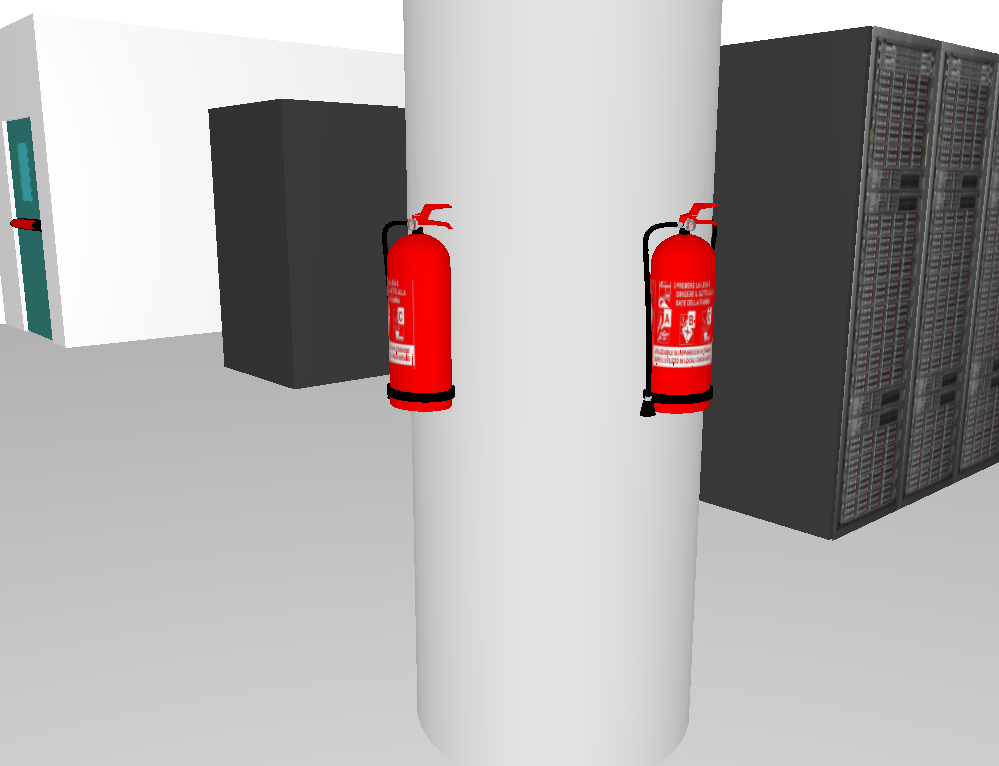
\includegraphics[width=6cm]{images/20170223-estintore2} &
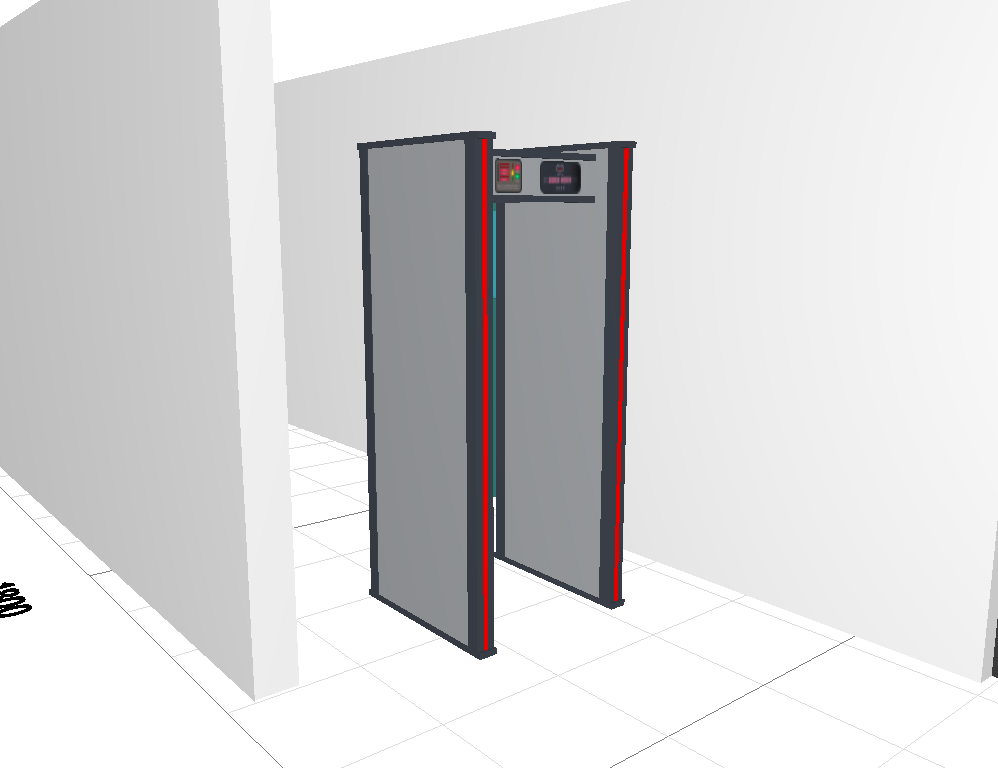
\includegraphics[width=6cm]{images/20170223-metaldetector2} \\
 (a) & (b) \\
\end{tabular}
\begin{tabular}{ccc @{\hspace{1em}} ccc}
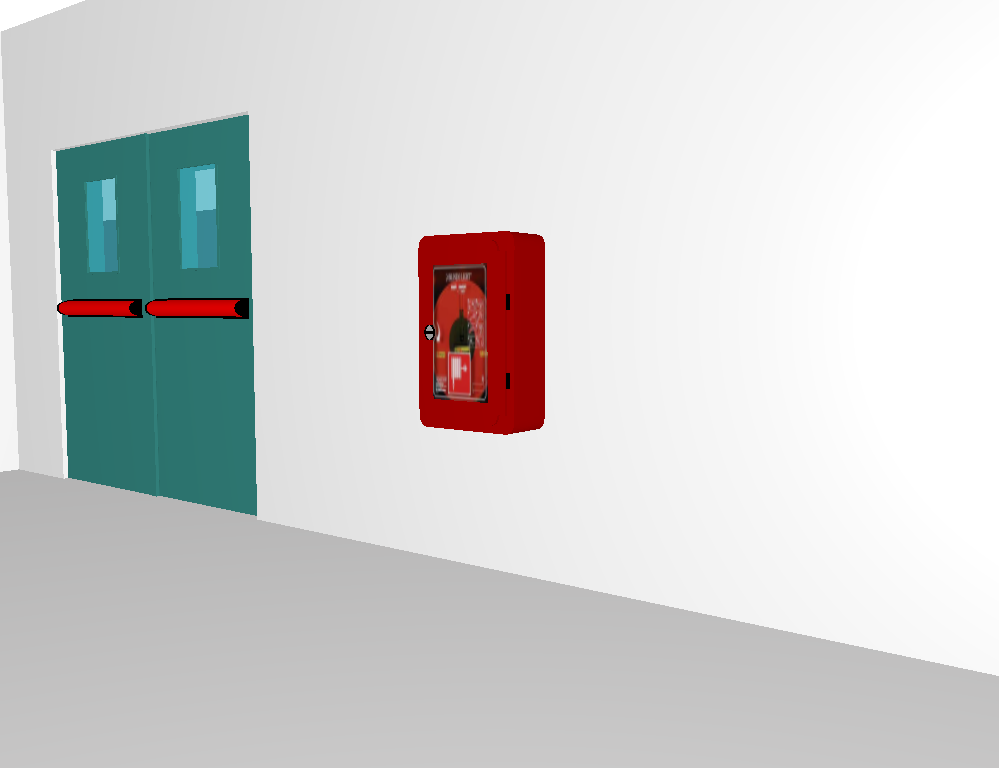
\includegraphics[width=4cm]{images/20170223-naspo2} &
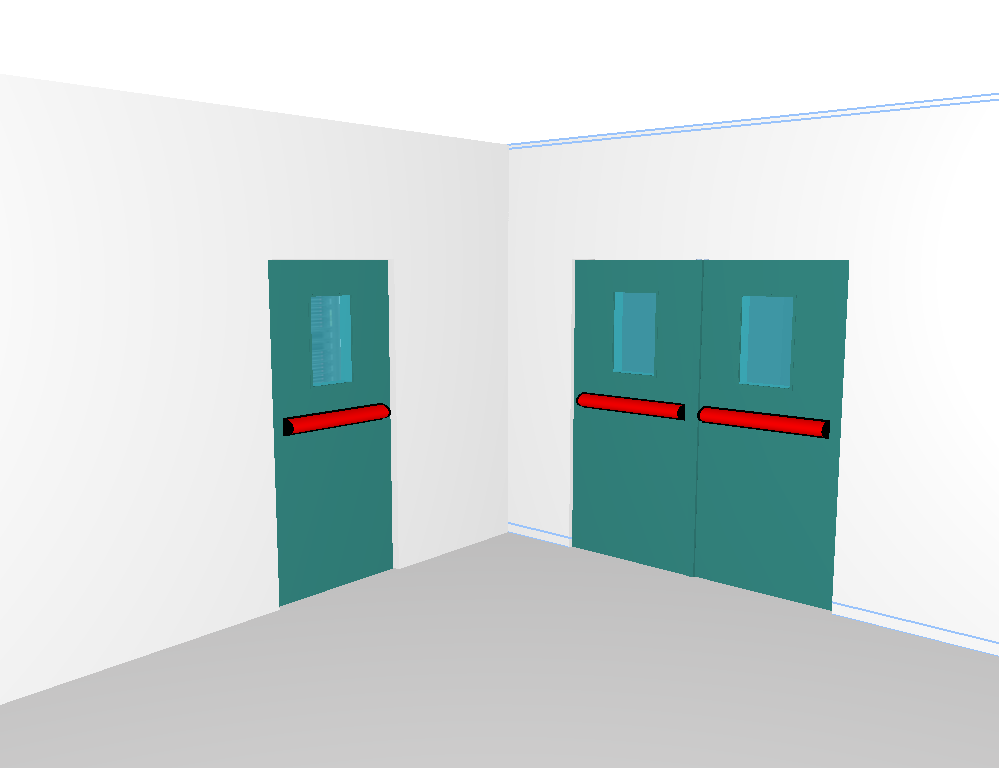
\includegraphics[width=4cm]{images/20170223-porta2} &
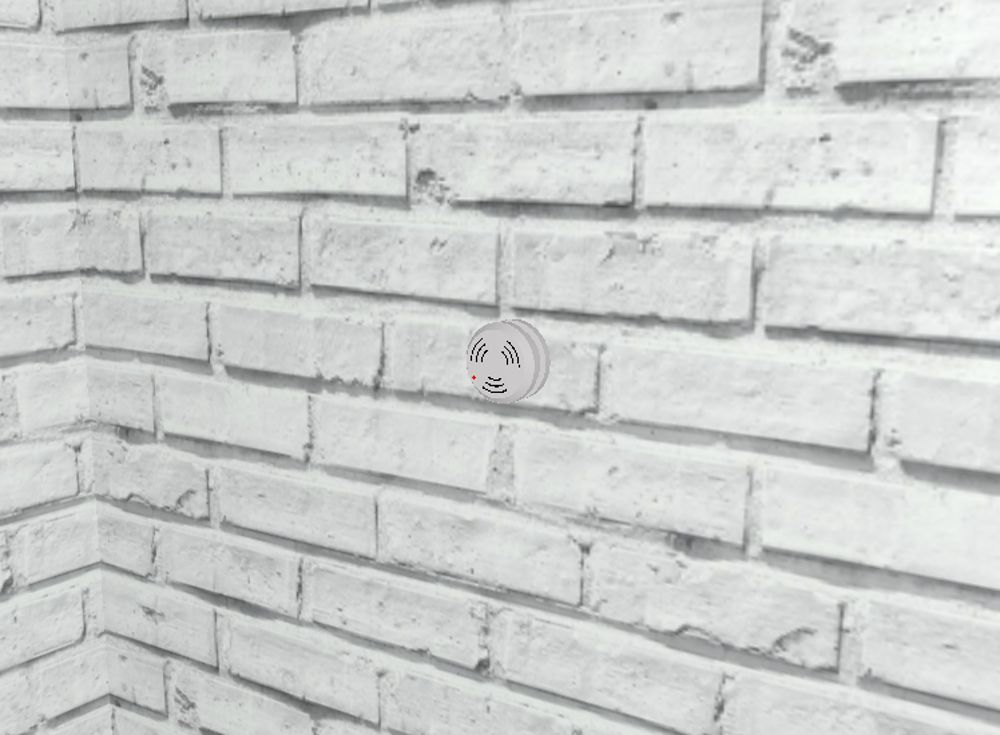
\includegraphics[width=4cm]{images/20170223-rilevatore2} \\
 (c) & (d) & (e)\\
\end{tabular}
\end{center}
\caption{Dettaglio Plugins: (a) estintore, (b) metal detecton, (c) rilevatore fumo, (d) cassetta naspo, (e) porta antipanico, (f) rilevatore di fumo}\label{fig:figura6}
\end{figure}
\newpage

Il secondo gruppo di \emph{Plugin} riguardano il contesto tecnologico (Figura~\ref{fig:figura7}), essi sono
un quadro elettrico, un rack server, un router wifi ed una telecamera. Questo gruppo ha un importanza rilevate in quanto
questi oggetti possono consentire un accesso remoto ed essere categorizzati come dispositivi \emph{IoT}.\\
\begin{figure}[htbp]
\begin{center}
\begin{tabular}{cc @{\hspace{1em}} cc}
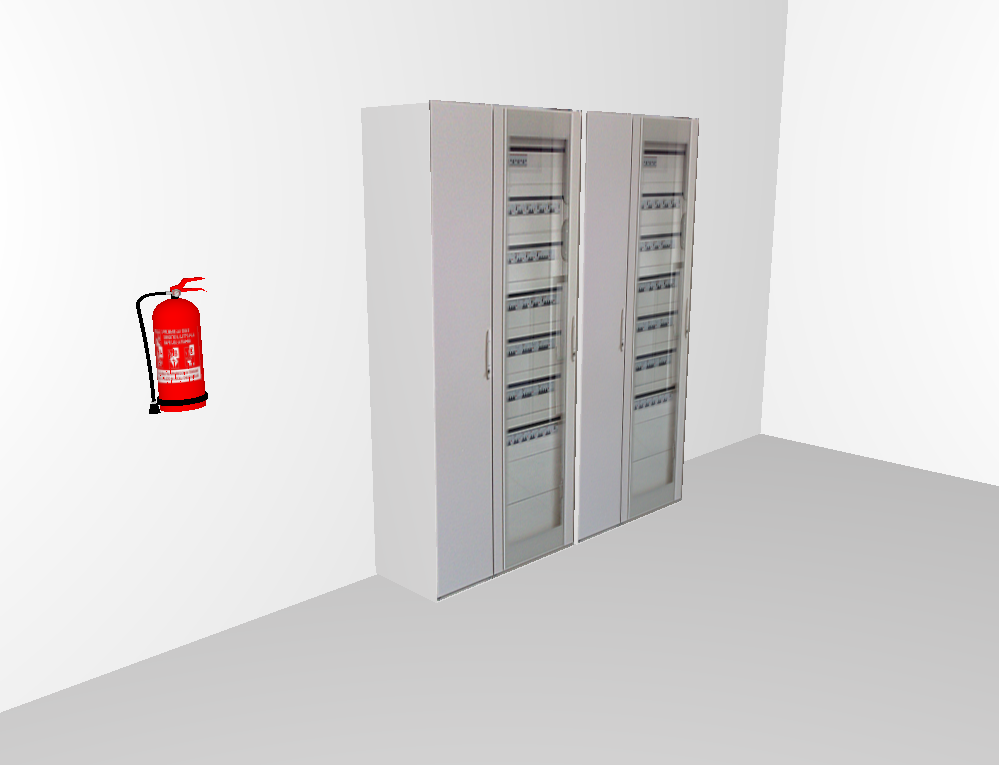
\includegraphics[width=6cm]{images/20170223-quadro2} &
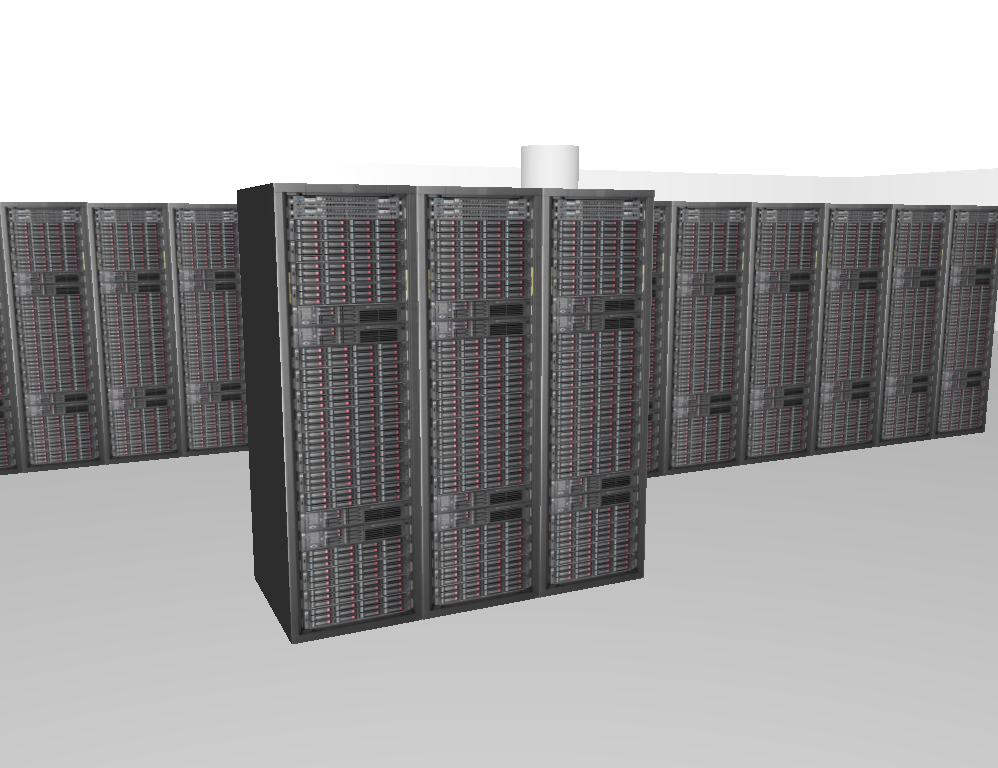
\includegraphics[width=6cm]{images/20170223-rack2} \\
 (a) & (b) \\
\end{tabular}
\begin{tabular}{cc @{\hspace{1em}} cc}
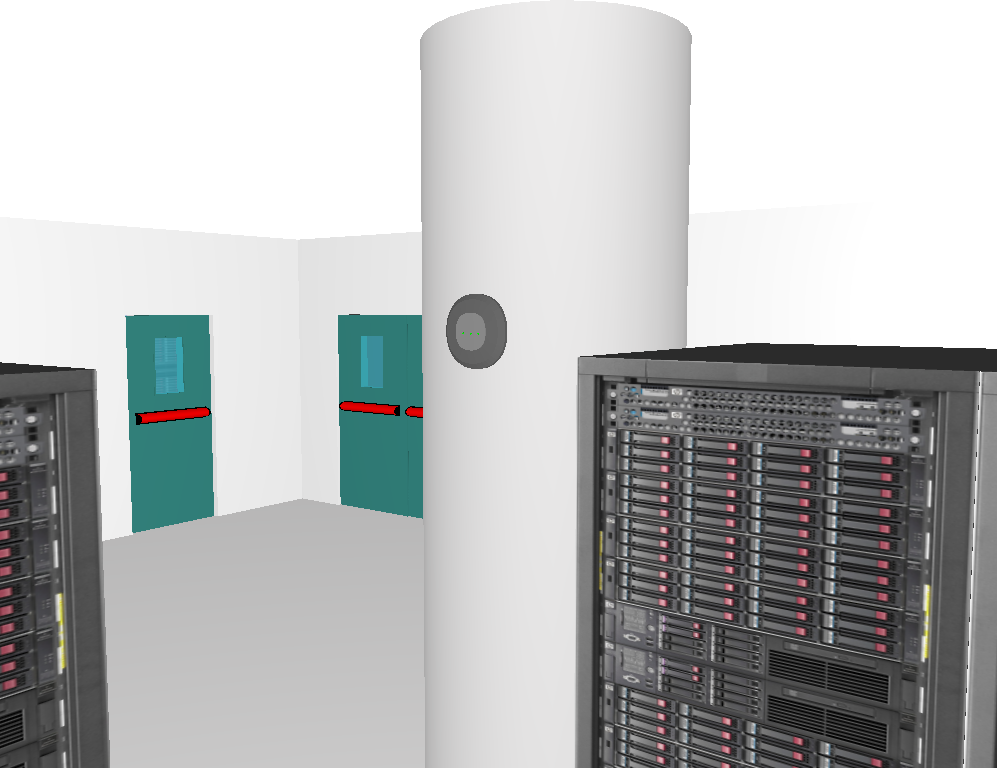
\includegraphics[width=6cm]{images/20170223-wifi2} &
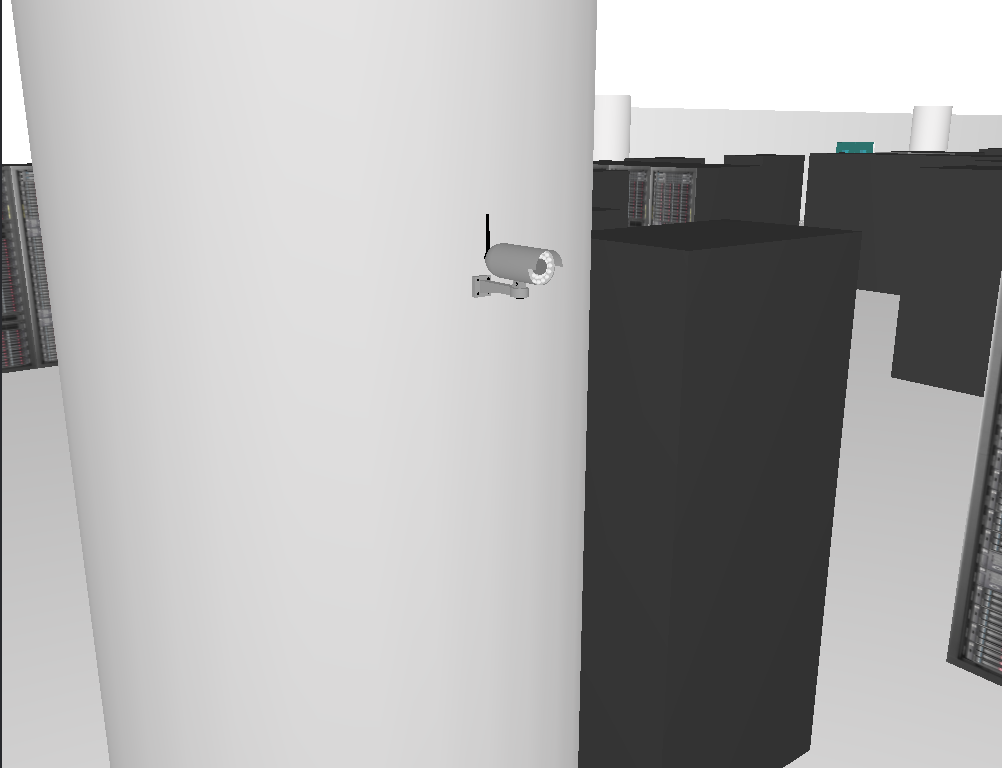
\includegraphics[width=6cm]{images/20170223-telecamera2} \\
 (c) & (d) \\
\end{tabular}
\end{center}
\caption{Dettaglio Plugin: (a) quadro elettrico, (b) rack server, (c) router wifi, (d) telecamera}\label{fig:figura7}
\end{figure}
\newpage
